\chapter{Conclusions and Recommendations}\label{chap:conclusions}
\section{Summary}
In this thesis we investigated new methods for computing the target photometric variables based on \textit{phase space ray tracing}. The aim was to understand how light propagates through non-imaging optical systems in order to calculate the target photometric variables, e.g., luminance and intensity. 
The core of this work was to use the \textit{phase space} which provides a full description of geometric optics. In this thesis we restricted ourselves to two-dimensional optical systems the phase space of which is a two-dimensional space. For every ray traced inside the system its path can be considered where a path is the sequence of the optical lines that it encounters. The phase space representation of the optical system shows that all the rays that follow the same path are located inside the same patch in phase space which is therefore divided into regions. Our idea was to determine the boundaries of those regions to obtain the photometric variables. In particular, assuming a Lambertian source, the coordinates of the rays located on the boundaries give all the information needed to compute the output luminance and therefore the intensity.
To this purpose, we developed two methods: phase space ray tracing and backward ray mapping in phase space. The goal of both is to trace only the rays close to the boundaries reducing the total number of rays traced compared to existing methods, for example Monte Carlo (MC) and Quasi-Monte Carlo (QMC) ray tracing.
\\ \\ \indent Phase space ray tracing exploits the phase space of the source and the target of the optical system. %In Chapter \ref{chap:PS} 
We introduced a procedure to construct a triangulation on the source phase space which allows tracing more rays close to the boundaries than to the interior of the positive luminance regions. 
The boundaries of those regions were approximated using two different approaches: the $\alpha$-shapes method and a technique based on the triangulation refinement. \\ \indent 
The $\alpha$-shapes relies on a parameter $\alpha$ which establishes which triangles have to be kept in the PS triangulation and which have to be removed to approximate the boundaries correctly. We developed a procedure based on \'{e}tendue conservation to determine the value of $\alpha$ that gives a good approximation of the boundaries.
%The $\alpha$-shape method was explained in Chapter \ref{chap:boundaries_alpha} and 
Numerical results were provided for two different kinds of TIR-collimators showing that phase space ray tracing using $\alpha$-shapes is much faster and more accurate than MC ray tracing. However, we observed that the speed of convergence depends on the smoothness of the shape of the regions in target phase space and, therefore, on the optical system. \\ \indent To eliminate the parameter $\alpha$ from the calculation of the boundaries, we developed a new approach for the boundaries computation based on the triangulation refinement. 
%explained in Chapter \ref{chap:triangulation}. 
This technique is able to determine the boundary triangles (triangles crossed by at least a boundary) of a given triangulation. Connecting the vertices of the boundary triangles corresponding to the rays that follow the same path, a good approximation of all the boundaries is obtained. Tracing more rays leads to smaller triangles resulting in a better accuracy of the boundaries computation. The stopping criterion employs \'{e}tendue conservation. 
The method was applied to several optical systems with reflective and refractive optical lines. The results show that the boundaries of all the regions with positive luminance in target PS are calculated correctly even for complicated systems such as the parabolic reflector for which multiple reflections of the rays with the mirrors can occur. Assuming a Lambertian source, the intensity was computed considering only the coordinates of the rays on the boundaries. 
The intensity profile obtained using phase space ray tracing based on the triangulation refinement is compared to the two intensities found with MC and QMC ray tracing. Phase space ray tracing allows tracing far less rays compared to MC ray tracing resulting in a significant reduction of the computational time. Our method has an order of convergence proportional to the reciprocal of the number of rays traced versus an error convergence proportional to the inverse of the square root of the number of rays traced for MC ray tracing. The results showed that PS ray tracing and QMC ray tracing are comparable in terms of the computational time, indeed the corresponding convergence errors are proportional to the inverse of the number of rays traced. For example the TIR-collimator, phase space ray tracing outperforms also QMC ray tracing while it is slower than QMC for some other systems as, for example, the parabolic reflector. However, we proved in simulations that PS ray tracing is binning free while MC and QMC errors depends on the number of bins in which the target is divided.
In order to further improve the phase space ray tracing we developed a second method which allows tracing only the rays located exactly on the boundaries of the regions with positive luminance. 
\\ \\ \indent The key idea of backward ray mapping was to construct an inverse map from the target to the source connecting the coordinates of the rays on the phase space of each optical line encountered. \\ \indent 
%In Chapter \ref{chap:raymapping1} 
We presented concatenated backward ray mapping valid for systems formed by straight line segments. It considers \textit{all} the lines that form the system. We showed that the boundaries of the regions that form every phase space can be calculated \textit{analytically}. Therefore, assuming a Lambertian source, concatenated backward ray mapping calculates the intensity \textit{exactly}. Compared to QMC ray tracing the method is much more accurate and also faster (the exact intensity was found in less time than QMC). 

%In Chapter \ref{chap:raymapping2} 
Next, we introduced direct backward ray mapping which is an extension of concatenated backward ray mapping to systems formed by curved lines. In this case the boundaries of all the phase spaces cannot be calculated analytically, therefore a bisection procedure combined with the inverse ray tracing is developed for computing the boundaries of the regions with positive luminance in phase space. As a consequence the \textit{exact} target intensity cannot be obtained for systems formed by curved lines. Nevertheless, the method remains very accurate and numerical results showed that it is also able to detect \textit{unphysical} paths due to numerical error where we referred to physical paths as those from the source to the target. Direct backward ray mapping provides a more accurate intensity distribution in less time compared to QMC ray tracing. To achieve an error of around $10^{-6}$, direct backward ray mapping is $10^3$ times faster than QMC ray tracing for the TIR-collimator and $10^2$ times faster than QMC ray tracing for the parabolic reflector. In Figure \ref{fig:error_comparison} we show an error comparison between all the methods applied to the TIR-collimator (left figure) and the parabolic reflector (right figure). 
We remark that while MC and QMC ray tracing are binning procedures which compute the averaged intensity, PS ray tracing and direct backward ray mapping compute the intensity pointwise. To compare the methods we calculated the averaged intensities also for PS ray tracing and direct backward ray mapping. Therefore, also for the PS procedures the target was divided into bins and the mean value of the intensity over every bin was computed. This mean value was given by the integral of the intensity over every bin divided by the size of the bin. In the simulation showed in this thesis, the integral was approximated using the trapezoidal rule discretizing the bin into $10$ more intervals of the same length. As a result, the CPU-time of the PS methods has to be divided by $10$ to obtain the real CPU-time when the PS methods are not compared with binning procedures.
\begin{figure}[h]
\label{fig:error_comparison}
 \begin{subfigure}[t]{0.49\textwidth}
\centering
    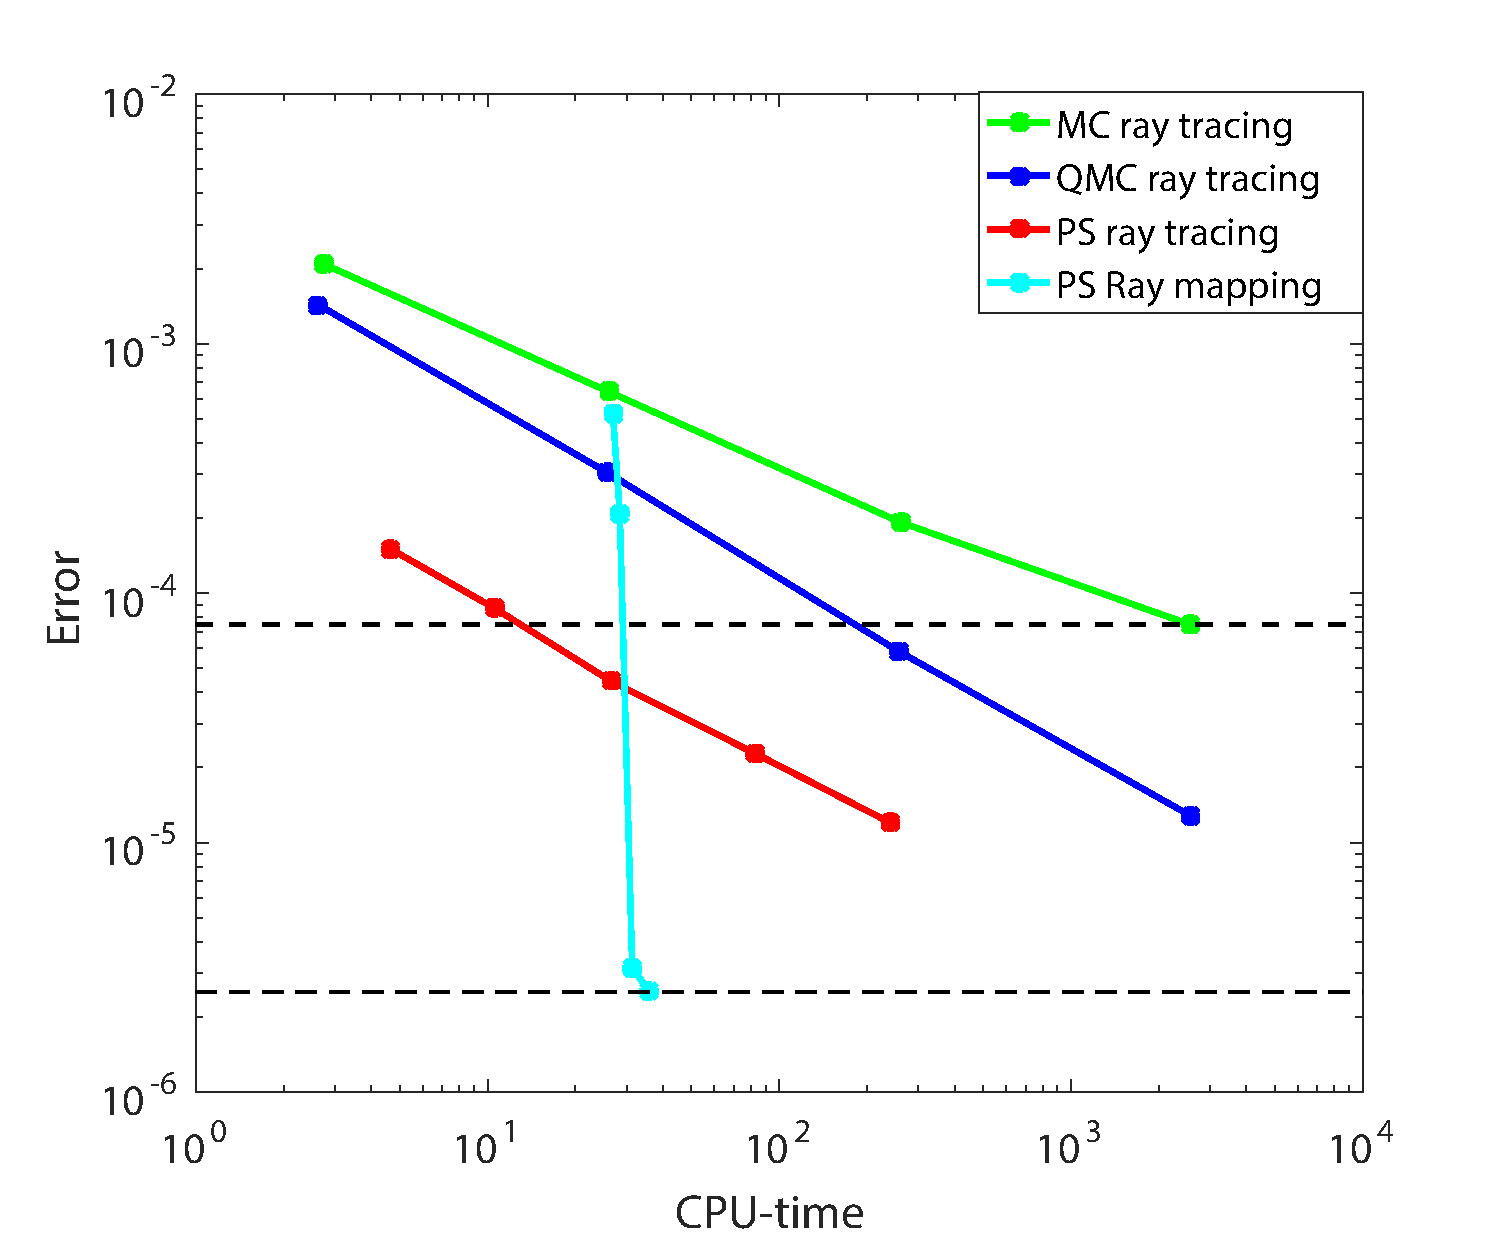
\includegraphics[width = \textwidth]{error_time_tir_all_methods}
    \caption{Error plot for the TIR-collimator.}
\end{subfigure}
\hfill
\begin{subfigure}[t]{0.49\textwidth}
\centering
    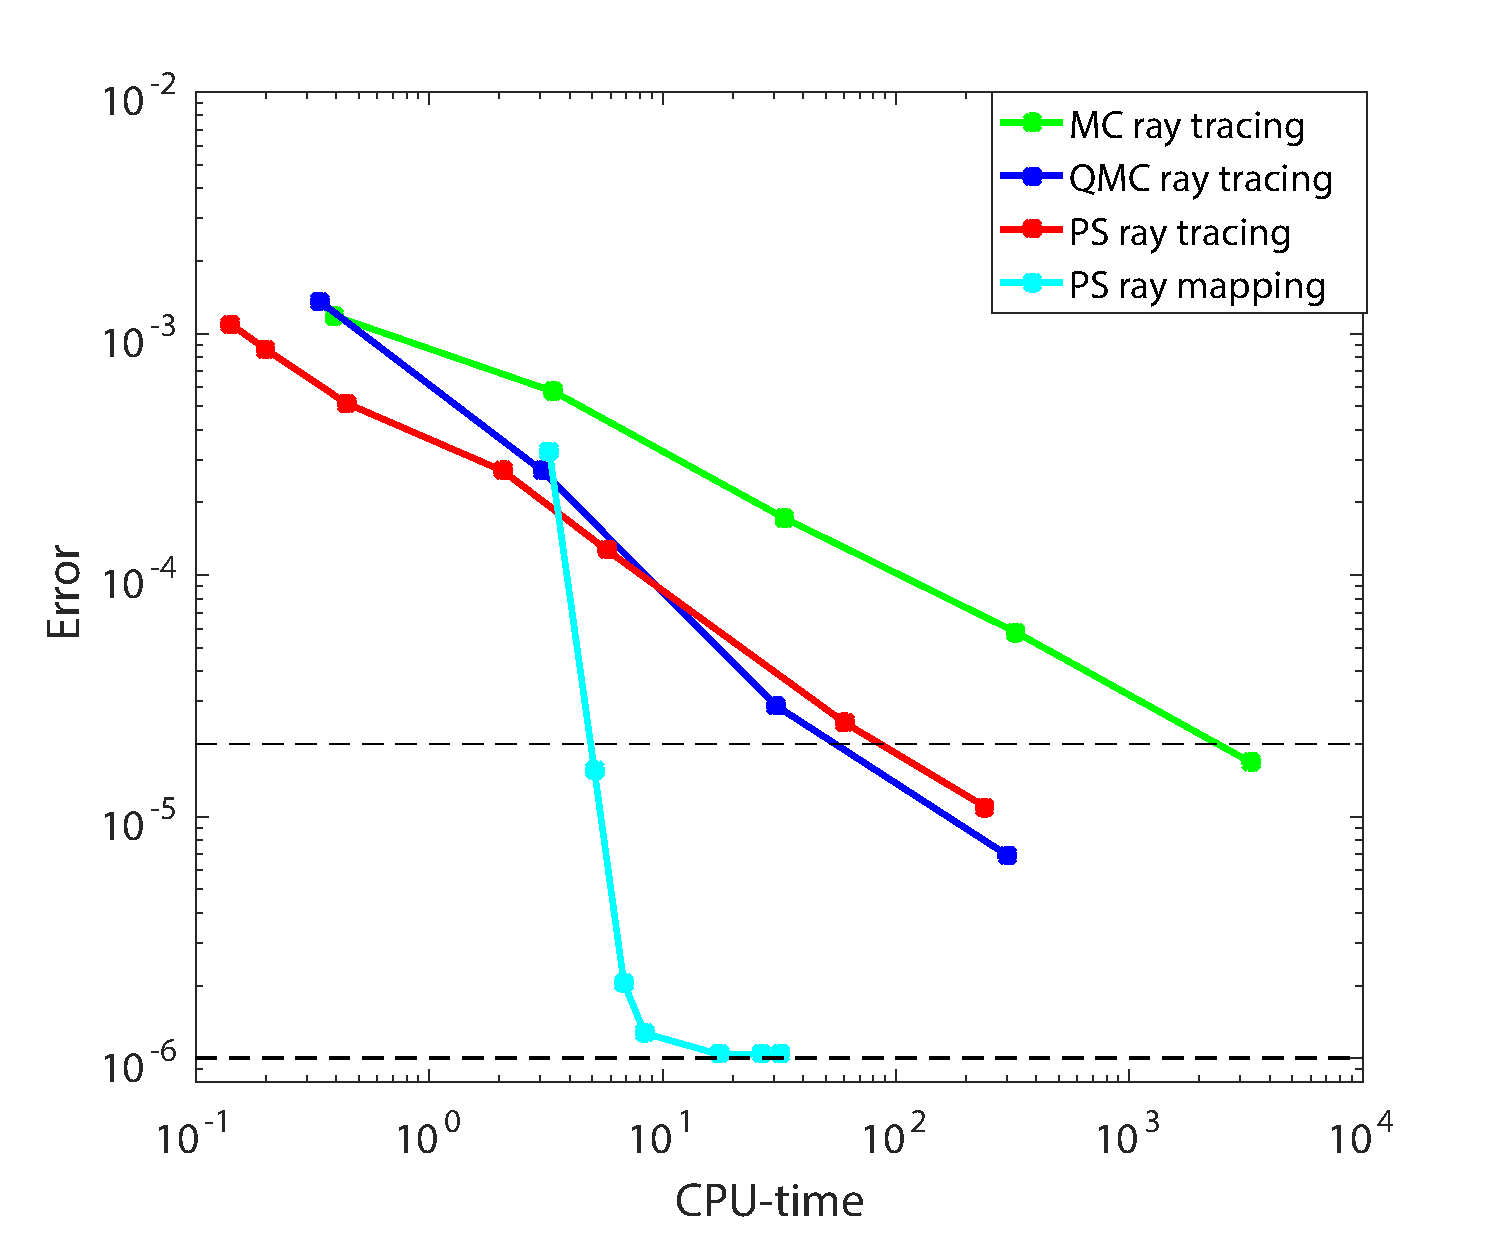
\includegraphics[width = \textwidth]{error_time_pr_all_methods}
    \caption{Error plot for the parabolic reflector.}
\end{subfigure}
\caption{\textbf{Comparison between MC, QMC, PS ray tracing and direct backward ray mapping.}}
\label{fig:error_comparison}
\end{figure}
\\ \indent
%in Chapter \ref{chap:fresnel}
Finally, we investigated systems where also Fresnel reflections were involved. Fresnel leads to multiple paths due to the fact that, at every interaction with a line, each ray is split in two rays (reflected and the transmitted) each of them carries a fraction of the energy transported by the incident ray. Direct backward ray mapping is able to detect \textit{all} the possible paths that can occur. Moreover, we showed that only the rays located on the boundaries of the regions in target phase space related to the \textit{physical} paths are traced from the target to the source. To validate our method we traced forward a set of rays using MC ray tracing and we showed that the boundaries found with direct backward ray mapping encompass all the rays traced. The power of energy associated to each ray on the boundary is calculated. For Fresnel systems the output luminance is not constant as depends on the angles of incident ray on every line and on the path followed by each ray. Therefore a sample of rays inside the regions with positive luminance needs to be traced back to compute the luminance and the intensity for optical systems with Fresnel reflections and refraction.
\\ \\ \indent To conclude we claim that phase space methods might constitute alternative approaches to conventional ray tracing. The advantages are that far less rays are needed for computing the target photometric variables resulting in a reduction of the computational time. In particular, phase space ray tracing is very easy to implement and faster than MC ray tracing. For some systems it outperforms also QMC ray tracing while for some others the boundaries of the positive luminance regions could be difficult to approximate and more rays are required. Because of this, in some cases phase space ray tracing can be slightly slower than QMC ray tracing. Direct backward ray mapping can be seen as an improvement of phase space ray tracing as it is much more accurate. It allows tracing far less rays compared to MC, QMC and PS ray tracing directly determining the rays on the boundaries of the positive luminance regions. Direct inverse ray mapping is a very elegant method and, compared to MC and QMC ray tracing it is faster and more accurate. This method could be used also to detect and minimize ghost stray light. The drawback of direct inverse ray mapping is that it is difficult to implement.
\section{Recommendations}
%For every boundary and along every direction, a sample of rays with position coordinates located between the rays on the boundaries need to be traced back in order to obtain the profile of the partial luminance along every direction. The total luminance is the sum of all the partial luminance related to each path. Finally the intensity cou 
%\\ \\ \indent In this thesis we showed that phase space is a powerful concept that fully characterize the optical systems. We presented two new methods based on phase space which allow traced far less rays than existing procedures to obtain the desired accuracy. This results in a significant reduction of the computational time. We evaluated the method for several optical systems in two-dimensions.
This work is far from finished. In the future, it might be useful to investigate in more details the two-dimensional case. The two-dimensional case is particularly relevant because is a good test for new methods. Moreover it gives a complete analysis of three-dimensional rotationally symmetric systems as it given a full description of the meridional plane.\\ \indent 
Regarding phase space ray tracing, could be interesting to analyze systems with a non Lambertian source. Our insight is to calculate the boundaries as we have done for a Lambertian source. Then the profile of the luminance can be obtained by tracing a sample of rays with corresponding coordinates located inside the boundaries found. The intensity can be obtained by merely integrating the luminance over all the possible positions. \\ \indent 
Regarding direct backward ray mapping we are interested in providing simulations for calculating the intensity profile also for systems with Fresnel reflection. The results shown in Chapter \ref{chap:fresnel} give the expectation that the direct backward ray mapping method is suitable also for such systems and that it is much more precise and faster than both MC and QMC ray tracing. Scattering phenomena could be described by generalizing direct backward ray mapping for Fresnel systems. More paths would occur as at every intersection each ray can be split in more than two rays as it scatters in multiple direction. However, we expect that the same algorithm can be used for every single path. 
%Furthermore colour
 \\ \indent 
Future research should address the three dimensional case. The first step could be to consider rotationally symmetric optical systems, i.e., systems invariant under rotations with respect to the optical axis. Such systems are often used in illumination optics as they are easy to manufacture. They can be described by only considering the meridional rays, that is rays that propagate inside the plane containing the optical axis. This reduces the three dimensional case to the two-dimensional one. 
For rotationally symmetric systems phase space ray tracing might constitute design tool for optical designers, greatly reducing the time to design the optical systems. 
\\ \indent  Next, it can be useful to analyze asymmetric optical systems \cite{ries1997performance}. Every ray is described by three position and two direction coordinates. The corresponding PS is therefore a four dimensional space described by two of the position coordinates $\variabile{q}_1$ and $\variabile{q}_2$ of the intersection point between the ray and the optical surface and two direction coordinates $\variabile{p}_1$ and $\variabile{p}_2$ expressed with respect to the normal of the surface. 
The target luminance in PS is a function of all these coordinates, while the intensity only depends on the direction coordinates and is given by a two-dimensional integral of the luminance over all the position coordinates $\variabile{q}_1$ and $\variabile{q}_2$. 
Therefore, for fixed directions $\variabile{p}_1$ and $\variabile{p}_2$, we need to compute the boundaries of the regions in the $(\variabile{q}_1, \variabile{q}_2)$-plane. In PS line in the two-dimensional case will become a surface in the three-dimensional case. 

To clarify our idea, we report a picture of the structure of the target of a three dimensional system showed in \cite{winston2005nonimaging} by Winston, Mi\~nano and Benitez.
In particular, they show the target of a CPC seen from above (constant direction). For example, Figures \ref{fig:melettaC} show the regions at the target of rays that leave the source with a given angle. The regions labeled $0, 1, 2,$... correspond to the regions that arrive at the target after after $0, 1, 2, \cdots$ reflections; $F2, F3,$... indicate the regions of the rays that begin to turn back after two, three, $\cdots$ reflections. The blank regions are formed by the rays that
still be traveling toward the exit aperture after five reflections. 
\begin{figure}[h]
\centering
    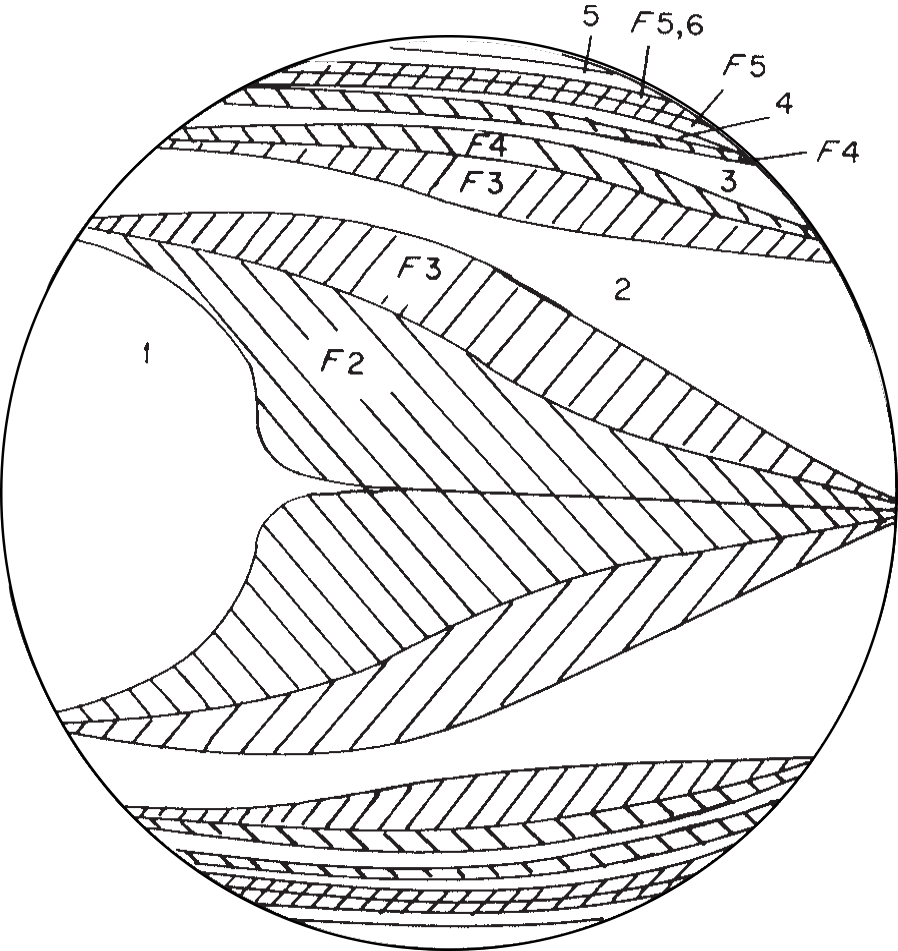
\includegraphics[width = 0.6\textwidth]{MelettaD}
    \caption{Regions at the target of a CPC of rays that leave the source with a fixed direction found using ray tracing. \cite{winston2005nonimaging}.}
\label{fig:melettaC}
\end{figure}
%In target PS the luminance is positive inside four dimensional objects. Hence the $2$D positive luminance regions at the target PS of two-dimensional systems become $4$D objects at the target PS of three-dimensional systems. The intensity along fixed directions $(\variabile{p}_1, \variabile{p}_2)$ is given by the integral of the luminance over all the possible positions $(\variabile{q}_1, \variabile{q}_2)$. Assuming a Lambertian source, we only need to compute the rays located on the boundaries of the $4$D positive luminance regions. Those boundaries are now surfaces instead of lines. Phase space ray tracing should deal with $5$-cell, that is a four-dimensional object bounded by $5$ tetrahedra cells. The boundaries of the regions with positive luminance (now triangular faces instead of lines) can be approximated either using four-dimensional $\alpha$-shapes (see for instance \cite{cazals2005conformal, teichmann1998surface}) or considering those triangular faces of each tethraedron located on one side of the boundaries of the region corresponding to a given path. Using the edge-ray principle the target boundaries are found and, therefore, the target photometric variables can be computed. Although the three-dimensional case will imply a more complicated structure of the PS and of the algorithm for surface reconstruction, we believe that phase space ray tracing is suitable in three dimensions. 
%We expect that for the boundaries reconstruction based on the triangulation refinement the speed of convergence will remain proportional to the inverse of the square root of the number of rays traced as every time that the tethraeda are halved the difference between the approximated \'{e}tendue at the target and the real \'{e}tendue should half.
%%
%\\ \indent 
%On the other hand, direct backward ray mapping extended to three-dimensional systems would be more complicated in a four dimensional target PS. Our idea is to discretize the hypercube into planes fixing both direction coordinates. Next, the bisection procedure can be applied fixing one of the two position $\variabile{q}_2$ coordinates and varying the other $\variabile{q}_1$. Repeating the procedure for all the possible values of $\variabile{q}_2$ would allow tracing back the rays located on the boundaries of the regions with positive luminance in the plane $(\variabile{q}_1, \variabile{q}_2)$ for fixed directions. In case of non Lambertian source, the luminance along those directions can be obtained tracing back a sample of rays inside those regions. Varying the direction coordinates $(\variabile{p}_1, \variabile{p}_2)$ and repeating the procedure for all the possible directions, the luminance can be calculated. The intensity profile is finally obtained by a two-dimensional integral over all the possible position coordinates. 
%\\ \indent 

We expect that both methods presented in this thesis can be extended to the three-dimensional case. Althought, the results showed for the two-dimensional case are very promising, we cannot predict the speed of convergence for the three-dimensional asymmetric optical systems. We expect that this would depend on the complexity of optical devices and of the corresponding regions in target PS. More research should be oriented on this topic.
